\documentclass[a4paper,10pt]{article}
\usepackage[utf8x]{inputenc}
\usepackage[brazil,brazilian]{babel}
\usepackage{graphicx}
\usepackage{listings}
%\usepackage{hyperref}

%\usepackage[autoplay=true]{movie15}
%\usepackage{animate}

\usepackage[hyphens]{url}
\usepackage[pdfauthor={Fabio Caritas Barrionuevo da Luz},%
breaklinks,pdftex]{hyperref}

%\hypersetup{
%    %colorlinks,%
%    citecolor=blue,%
%    filecolor=blue,%
%    linkcolor=blue,%
%    urlcolor=blue
%}




\usepackage{color}
 
\definecolor{dkgreen}{rgb}{0,0.6,0}
\definecolor{gray}{rgb}{0.5,0.5,0.5}
\definecolor{mauve}{rgb}{0.58,0,0.82}


\lstset{ %
  language=Python,                % the language of the code
  basicstyle=\footnotesize,           % the size of the fonts that are used for the code
  numbers=left,                   % where to put the line-numbers
  numberstyle=\tiny\color{gray},  % the style that is used for the line-numbers
  stepnumber=2,                   % the step between two line-numbers. If it's 1, each line 
                                  % will be numbered
  numbersep=5pt,                  % how far the line-numbers are from the code
  backgroundcolor=\color{white},      % choose the background color. You must add \usepackage{color}
  showspaces=false,               % show spaces adding particular underscores
  showstringspaces=false,         % underline spaces within strings
  showtabs=true,                 % show tabs within strings adding particular underscores
%  frame=single,                   % adds a frame around the code
  frame=shadowbox,
  rulecolor=\color{black},        % if not set, the frame-color may be changed on line-breaks within not-black text (e.g. commens (green here))
  tabsize=2,                      % sets default tabsize to 2 spaces
  captionpos=b,                   % sets the caption-position to bottom
  breaklines=true,                % sets automatic line breaking
  breakatwhitespace=false,        % sets if automatic breaks should only happen at whitespace
  title=\lstname,                   % show the filename of files included with \lstinputlisting;
                                  % also try caption instead of title
  keywordstyle=\color{blue},          % keyword style
  commentstyle=\color{dkgreen},       % comment style
  stringstyle=\color{mauve},         % string literal style
  escapeinside={\%*}{*)},            % if you want to add a comment within your code
  morekeywords={*,...,., True, False, self}               % if you want to add more keywords to the set
}

\newcommand{\code}[2]{
  \hrulefill
  \subsection*{#1}
  \lstinputlisting{#2}
  \vspace{2em}
}




%\usepackage{framed}
%pacote para a criacao de automatos e grafos
%\usepackage{vaucanson-g}

%\lstset{frame=shadowbox, rulesepcolor=\color{blue}, breaklines=true}

\title{Uma Implementação dos Algoritmos para resolução do Problema do Caminho Mínimo}
\author{Fábio Cáritas Barrionuevo da Luz
\\\small{
\textit{Sistemas de Informação - }
\textit{Faculdade Católica do Tocantins}
}
}

\begin{document}

\maketitle
\tableofcontents
\begin{abstract}
\begin{center}
Este trabalho tem por objetivo relatar a experiência com implementação do Algoritmo de Dijkstra e Algoritmo de Bellman-Ford
\end{center}
\end{abstract}
\newpage

%\begin{section}{Introdução}
\section{Introdução}{
\begin{center}
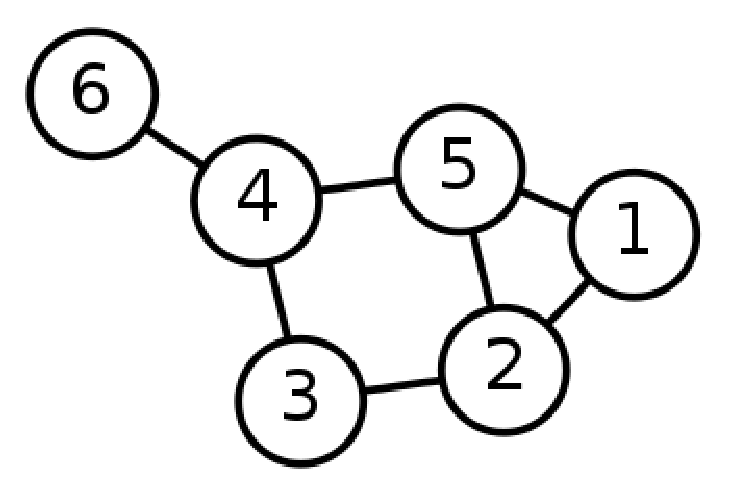
\includegraphics[width=3cm]{grafo_6v_7_arestas.eps}

\end{center}    
\begin{quotation}
Uma transportadora planeja fazer uma promoção de 50\% de desconto para aumentar seus negócios.
Só que para essa promoção não dar prejuízo, os caminhões devem passar somente pelas estradas de menor extensão.
Para tanto, a equipe de negócios da transportadora deve descobrir quais são as rotas(percurso por estradas) de menor extensão que interligam todas as suas filiais.\\
Mas há um problema, a transportadora possui 500 filiais, e existem mais de 5000 estradas diferentes que interligam direta e indiretamente todas essas 500 filiais.
Como descobrir quais as melhores Rotas?
\end{quotation}


Esse tipo de problema pode ser resolvido com a utilização de Grafos.
Um grafo é representado como um conjunto de pontos (vértices) que possuem ligação (as arestas).




Grafos podem ser utilizados para a resolução de diversos tipos de problemas, como por exemplo, o Grafo do Conhecimento\cite{1}\cite{2}, uma 
implementação do gigante de Buscas Google que visa melhorar a relevância do resultado das buscas relacionada a palavra chave pesquisada 
ou para o auxilio na gestão de tempo de projetos \cite{3}.

No caso do problema da transportadora, cada uma das 500 filiais representaria um vértice, e cada uma das estradas que interligam as filiais, representariam as arestas. 

Problemas desse tipo são classificados como  \textbf{``Problema do Caminho Mínimo''}.
O problema do caminho mínimo consiste na minimização do custo de travessia de um grafo entre dois vértices, custo este dado pela soma dos pesos ou custo de cada aresta percorrida.

Uma aresta representa a ligação entre dois vértices, esta ligação por ter custo e sentido.
Um Vértice pode representar o ponto de encontro de duas arestas.%\footnote[1]{Partes do texto retirados de: http://pt.wikipedia.com}

Os algoritmos mais conhecidos para resolução do ``Problema do Caminho Mínimo'' são o Algoritmo de Dijkstra\cite{4} e o algoritmo de Bellman-Ford\cite{5}

}

\section{Algoritmos de Dijkstra}{
    

 Algoritmos de Dijkstra\cite{4}, foi concebido pelo cientista da computação holandês Edsger Dijkstra[7] em 1956 e publicado em 1959, servindo para localizar todos os caminhos mínimos
de determinado vértice origem para todos os outros vértices alcançáveis do Grafo, somente se não houver caminhos(arestas) de custo negativo.


O Algoritmos de Dijkstra pode ser descrito da seguinte forma:
\begin{enumerate}
 \item \textit{Inicialização:}
 \\Criar dois vetores, ``distancia'' e ``anterior'', cujo o tamanho seja o numero de vértices do Grafo G e uma lista ``q'', que contenha todos os vértices pertencentes ao Grafo G.
 \\Em seguida para todo vértice v pertencente ao Grafo G, fazer com que o vetor ``distancia'' na ``posição v'' 
receba um valor muito alto, fazer com que ``anterior'' na ``posição v'' receba valor nulo.
Fazer com que ``distancia'' na posição ``vértice origem'' receba o valor 0.

 
  \item \textit{Processamento de Caminhos mínimos:}
 \\Enquanto lista ``q'' não estiver vazia, obter do vetor ``distancia'' o vértice ``u'' com menor custo somente se o vértice ``u'' estiver contido na lista ``q''.
 \\Remover o vértice ``u'' da lista ``q''.
 \\Para cada ``visinho'' do vértice ``u'' (vértice em que ``u'' possui ligação), obter a soma `soma` de vetor ``distancia'' na posição ``u'' mais o custo da ligação de ``u'' com ``visinho''.
 \\Se ``soma'' for menor do que vetor ``distancia'' na posição ``visinho'', fazer com que vetor ``distancia'' na posição ``visinho'' receba ``soma'' e vetor ``anterior'' na posição ``visinho'' receba ``u''.
  
\end{enumerate}

 Para se obter o o percurso mínimo de um vértice origem até o vértice destino, basta iterar sobre o vetor ``anterior'', começando da posição ``destino'' até quando vetor ``anterior'', na posição ``destino'' for nulo,
\begin{enumerate} 
  \item[3] \textit{Chegar ao destino}
  \\criar uma lista ``percurso'',
  \\Enquando  vetor ``anterior'' na posição ``destino'' não for nulo, adicionar vértice ``destino'' ao final da lista ``percurso''.
  \\Fazer com que ``destino'' receba vetor ``anterior'' na posição ``destino''
  \\Quando o vetor ``anterior'' na posição ``destino'' for nulo, adicionar vértice origem'' ao final da lista ``percurso''.
\end{enumerate}

Ao final da execução, a lista ``percurso'' conterá o caminho minimo partindo do vértice origem ate o vértice destino.
\begin{lstlisting}[morekeywords={*,:,:,[,], se, de, para, todo, fim para, enquanto, nao, eh, retorne}, captionpos=b]
funcao Dijkstra(Grafo, origem):
    // Inicializacao
    para todo vertice v em Grafo:
        distancia[v] := Numero_Muito_Grande ;
        anterior[v] := undefined ;
    fim para ;
    distancia[origem] := 0;
    Q :=lista de todos os vertices do Grafo ;
    //Inicio do processamento
    enquanto Q nao eh vazio:              
        u := vertice u de menor custo em distancia[] se u estiver contido em Q;   
        se distancia[u] = Numero_Muito_Grande:
            break ; // Todos os vertices que sobraram em q sao inacessiveis
        fim se ;
        remova u de Q ;
        para todo visinho v of u://para cada visinho de u que esta contido em Q
            soma := distancia[u] + distancia_entre(u, v) ;
            se soma < distancia[v]:  
                distancia[v] := soma ;
                anterior[v] := u ;
            fim se ;
        fim para ;
    fim enquanto ;
    retorne distancia[] e anterior[] ;
fim Dijkstra.
\end{lstlisting}

Obtendo o percurso entre o vértice origem e o vértice destino
\begin{lstlisting}[morekeywords={*,:,:,[,], se, de, para, todo, fim para, enquanto, nao, eh, retorne}, captionpos=b]
funcao caminho_minimo_entre_vertices(Grafo, origem, destino):
    distancia[], anterior[] = Dijkstra(Grafo, origem)
    lista percurso
    enquanto anterior[destino] nao for nulo, faca:
        adicione anterior[destino] ao final da lista percurso
        destino = anterior[destino]
    fim enquanto
    adicione origem ao final da lista percurso
    retorne percurso

fim funcao caminho_minimo_entre_vertices
\end{lstlisting}
%\code{Implementação}{caminho_minimo.py}

%\end{center}    
}


\section{Algoritmo de Bellman-Ford}{
 Algoritmos de Bellman-Ford\cite{5}, foi concebido pelo matemático americano Richard Ernest Bellman [9], servindo para localizar todos os caminhos mínimos
de determinado vértice origem para todos os outros vértices alcançáveis do Grafo, incluindo os \textbf{caminhos(arestas) de custo negativo}.

\begin{lstlisting}[morekeywords={*,:,:,[,], se, de, para, todo, fim para, enquanto, nao, eh, retorne}, captionpos=b]
funcao Bellman-Ford(Grafo, origem):

    // Inicializacao
    para todo vertice v em Grafo:
        distancia[v] := Numero_Muito_Grande ;
        anterior[v] := undefined ;
    fim para ;
    distancia[origem] := 0 ;

    //Inicio do processamento
    para i =1 ate numero total de vertices:
        para todo vertice u em Grafo:              
            para todo vertice v em Grafo:
                soma := distancia[u] + distancia_entre(u, v) ;
                se distancia[v] > soma:  
                    distancia[v] := soma ;
                    anterior[v] := u ;
                fim se ;
            fim para ;
        fim para ;
    fim para
    para todo vertice u em Grafo:              
        para todo vertice v em Grafo:
            soma := distancia[u] + distancia_entre(u, v) ;
            se distancia[v] > soma:
                retorne Falso
            fim se ;
        fim para ;
    fim para ;
    retorno Verdadeiro 
fim Bellman-Ford.
\end{lstlisting}
}

\section{Testes}{
A validação da implementação ocorreu com conjuntos de testes contendo 8, 50, 250, 500, 750 e 1000 nós, e
mais um com apenas 4 para verificar o tratamento de ciclo negativo.
O tempo de execução para cada algoritmo, métrica adotada e número de nós é exibido nas tabelas a seguir. Os
pontos de origem e destino são aleatórios para cada conjunto de nós.

A tabela 1 exibe os tempos de execução do algoritmo Bellman Ford e o caminho encontrado para cada conjunto
de nós.

\begin{center}
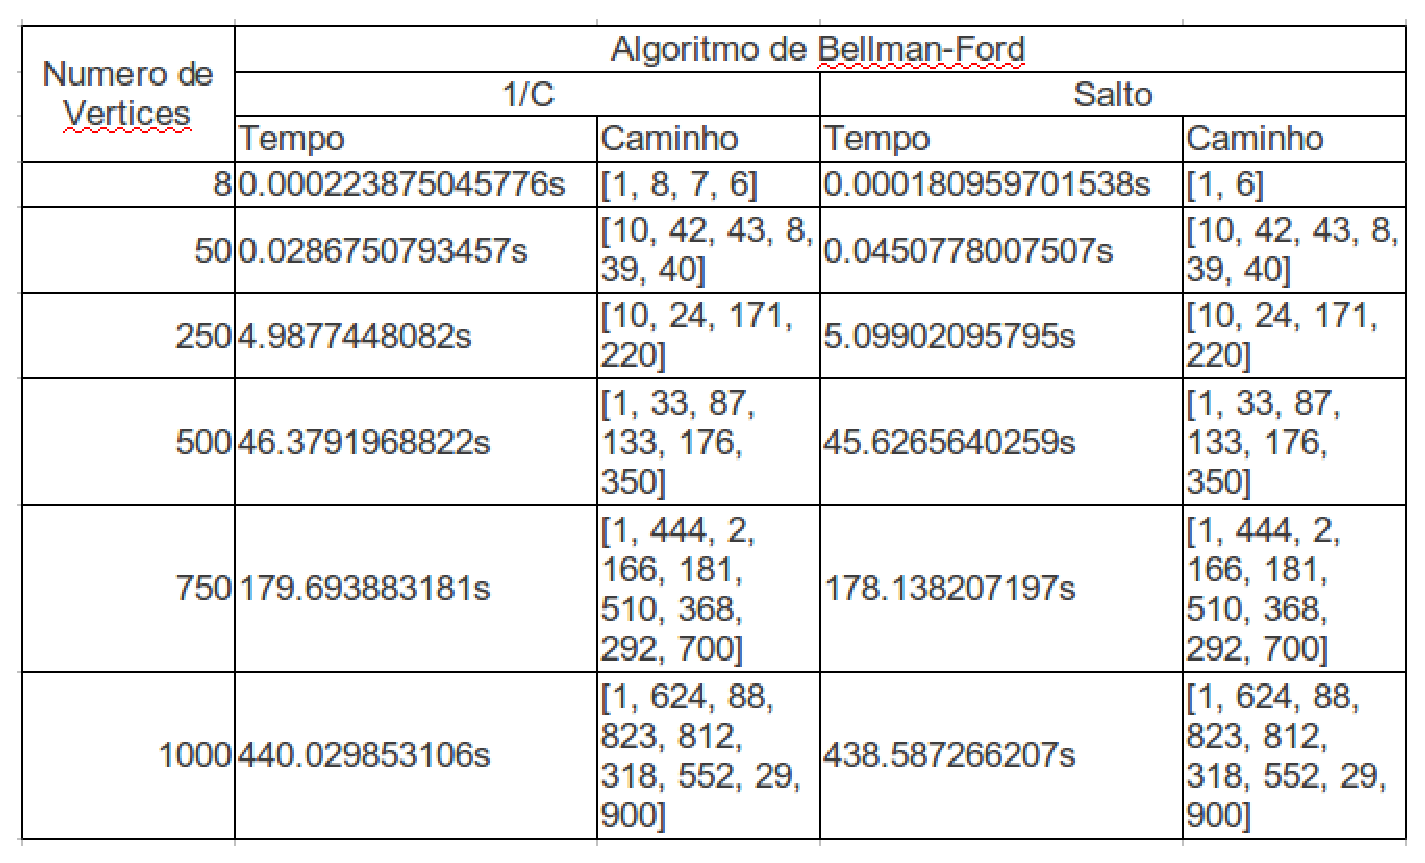
\includegraphics[width=13cm]{bellman_tab.eps}

\end{center}  


A tabela 2 exibe os tempos de execução do algoritmo Dijkstra e o caminho encontrado para cada conjunto de
nós.

\begin{center}
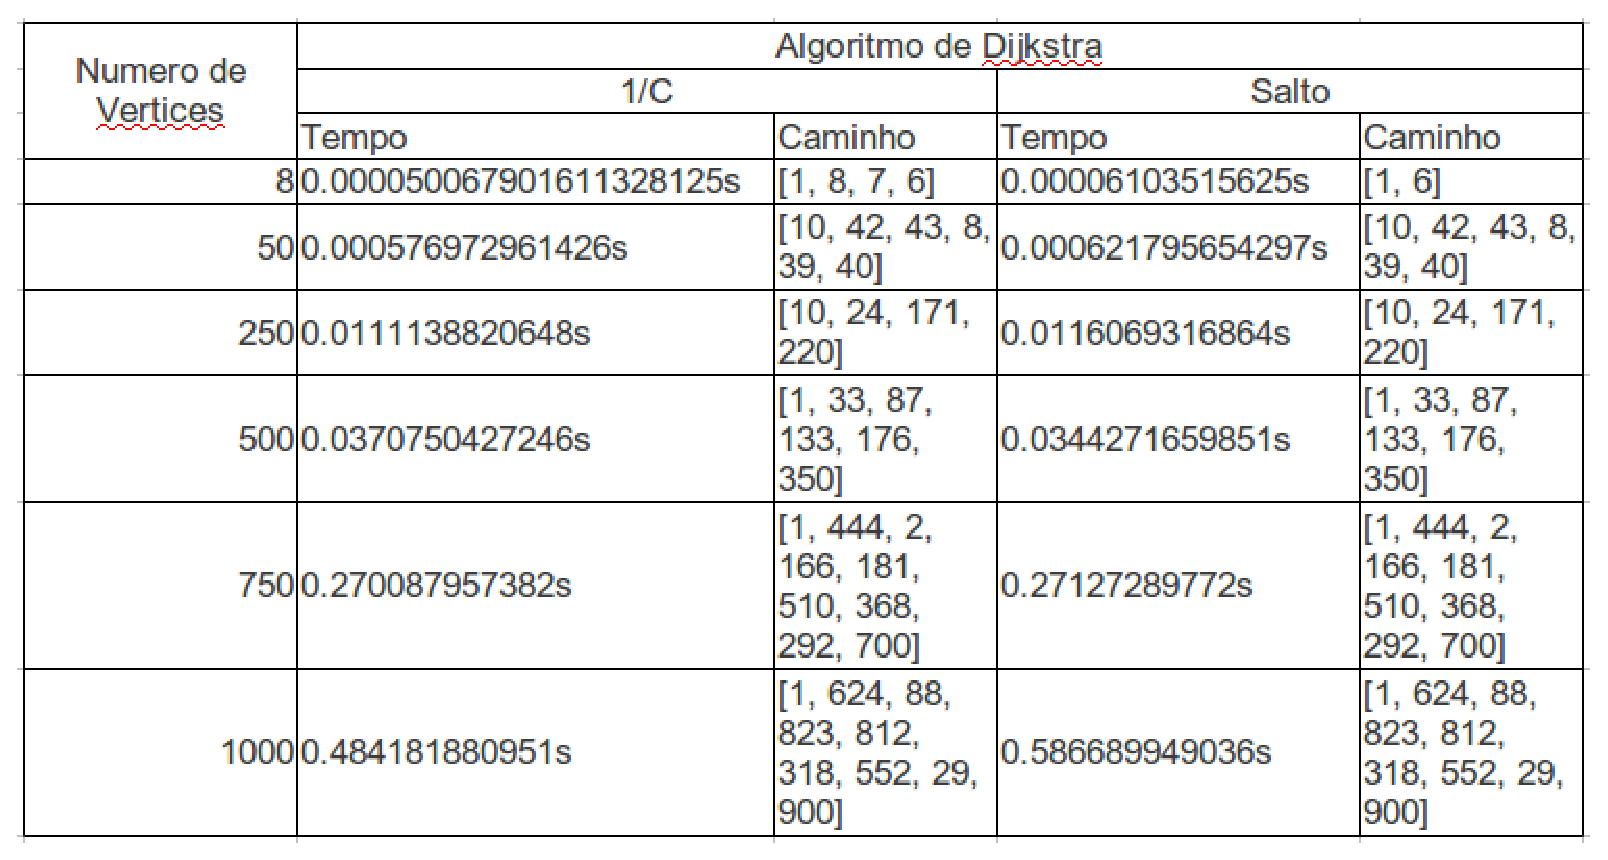
\includegraphics[width=13cm]{dijkstra_tab.eps}

\end{center}  


}


\section{Conclusão}{
Uma das principais diferenças entre os algoritmos estudados nessa disciplina é o fato de o Dijkstra não realizar
todas as comparações como é feito no Bellman-Ford. O primeiro realiza apenas o número de arestas, enquanto
o segundo realiza o número de todas as arestas por arestas.

}



\section{Bibliografia}{
 \begin{thebibliography}{9}
 \bibitem[1]{1} \emph{\href{http://goo.gl/bZyyN}{http://googlediscovery.com/2012/05/16/google-anuncia-grafo-do-conhecimento/}},  acessado em 24/05/2012

 \bibitem[2]{2} \emph{\href{http://www.youtube.com/watch?v=mmQl6VGvX-c}{Video apresentando o Grafo do Conhecimento:}}, http://www.youtube.com/watch?v=mmQl6VGvX-c acessado em 24/05/2012
 
 \bibitem[3]{3} \emph{\href{http://www.ufrrj.br/codep/materialcursos/gerenciamento/gerenciamentotempo/CGP-GT_PERT_CPM_FernandoNogueira.pdf}{ Fernando Nogueira- Notas de Aula - Disciplina de Pesquisa Operacional}}, - Estimativa de Três pontos - PERT/CMP - UFRRJ - Universidade Federal Rural do Rio de Janeiro ,acessado em 24/05/2012
 

 \bibitem[4]{4} \emph{Edsger W. Dijkstra. \href{http://www-m3.ma.tum.de/foswiki/pub/MN0506/WebHome/dijkstra.pdf}{``A note on two problems in connection with graphs''.}
 [S.l.]:. Numerische Mathematik 1, 1959. 83–89 p.},
    
 \bibitem[5]{5} \emph{Bellman, Richard (1958). \href{http://monet.skku.ac.kr/course_materials/undergraduate/al/lecture/2006/BellmanFord.pdf}{"On a routing problem".} },Quarterly of Applied Mathematics 16: 87–90.   
 

 \bibitem[6]{6} \emph{\href{http://pt.wikipedia.org/wiki/Algoritmo_de_Dijkstra}{Algoritmo de Dijkstra }}, - Wikipedia, acessado em 24/05/2012

 \bibitem[7]{7} \emph{\href{http://pt.wikipedia.org/wiki/Edsger_Dijkstra}{Edsger Wybe Dijkstra}},- Wikipedia, acessado em 24/05/2012

 \bibitem[8]{8} \emph{\href{http://pt.wikipedia.org/wiki/Algoritmo_de_Bellman-Ford}{Algoritmo de Bellman-Ford}},- Wikipedia, acessado em 24/05/2012

 \bibitem[9]{9} \emph{\href{http://en.wikipedia.org/wiki/Richard_E._Bellman}{Richard Ernest Bellman }},- Wikipedia, acessado em 24/05/2012
\end{thebibliography}
}

\section{Implementação em Python}{
\code{Implementação}{caminho_minimo.py}
}

\end{document}
